%%=============================================================================
%% Inleiding
%%=============================================================================

\chapter{Inleiding}
\label{ch:inleiding}

%De inleiding moet de lezer alle nodige informatie verschaffen om het onderwerp te begrijpen zonder nog externe werken te moeten raadplegen \autocite{Pollefliet2011}. Dit is een doorlopende tekst die gebaseerd is op al wat je over het onderwerp gelezen hebt (literatuuronderzoek).

%Je verwijst bij elke bewering die je doet, vakterm die je introduceert, enz. naar je bronnen. In \LaTeX{} kan dat met het commando \texttt{$\backslash${textcite\{\}}} of \texttt{$\backslash${autocite\{\}}}. Als argument van het commando geef je de ``sleutel'' van een ``record'' in een bibliografische databank in het Bib\TeX{}-formaat (een tekstbestand). Als je expliciet naar de auteur verwijst in de zin, gebruik je \texttt{$\backslash${}textcite\{\}}.
%Soms wil je de auteur niet expliciet vernoemen, dan gebruik je \texttt{$\backslash${}autocite\{\}}. Hieronder een voorbeeld van elk.

%\textcite{Knuth1998} schreef een van de standaardwerken over sorteer- en zoekalgoritmen. Experten zijn het erover eens dat cloud computing een interessante opportuniteit vormen, zowel voor gebruikers als voor dienstverleners op vlak van informatietechnologie~\autocite{Creeger2009}.

\section{Stand van zaken}
\label{sec:stand-van-zaken}

%% TODO: deze sectie (die je kan opsplitsen in verschillende secties) bevat je
%% literatuurstudie. Vergeet niet telkens je bronnen te vermelden!


De onderzoeken en technieken om de noden van gebruikers te voorspellen kent de laatste jaren een grote opmars. Google en Facebook zijn dan ook volop bezig met eigen onderzoekscentra en technologieën te ontwikkelen om aan Artificiële Intelligentie te doen. FAIR is de afkorting voor Facebook Artificial Intelligence Research. Er zijn wereldwijd 3 labo's die constant op zoek zijn naar nieuwe mogelijkheden binnen AI (Artificiële Intelligentie). RankBrain is een algoritme van Google die a.d.h.v. artificiële intelligentie de ranking van een bepaalde site op zoekpagina's bepaalt.
De persoonlijke advertenties die Google toont zijn veelal gegenereerd met algoritmes.  Maar ook gerelateerde producten of 'wat jou ook kan interesseren'-lijsten worden dikwijls door machine learning opgemaakt. Tensorflow \autocite{tensorflow} is een open source API ontwikkelt door Google die je uiteraard gratis kan gebruiken om zelf toepassingen met AI te maken. De API is ontwikkeld in Python. Deze taal is één van de veel gebruikte in de data science\autocite{pythonMostPopular}.

In deze bachelorproef zullen er voorspellingen gemaakt worden op een arcademachine (figuur \ref{fig:arcademachine}).
\begin{figure}
	\centering
	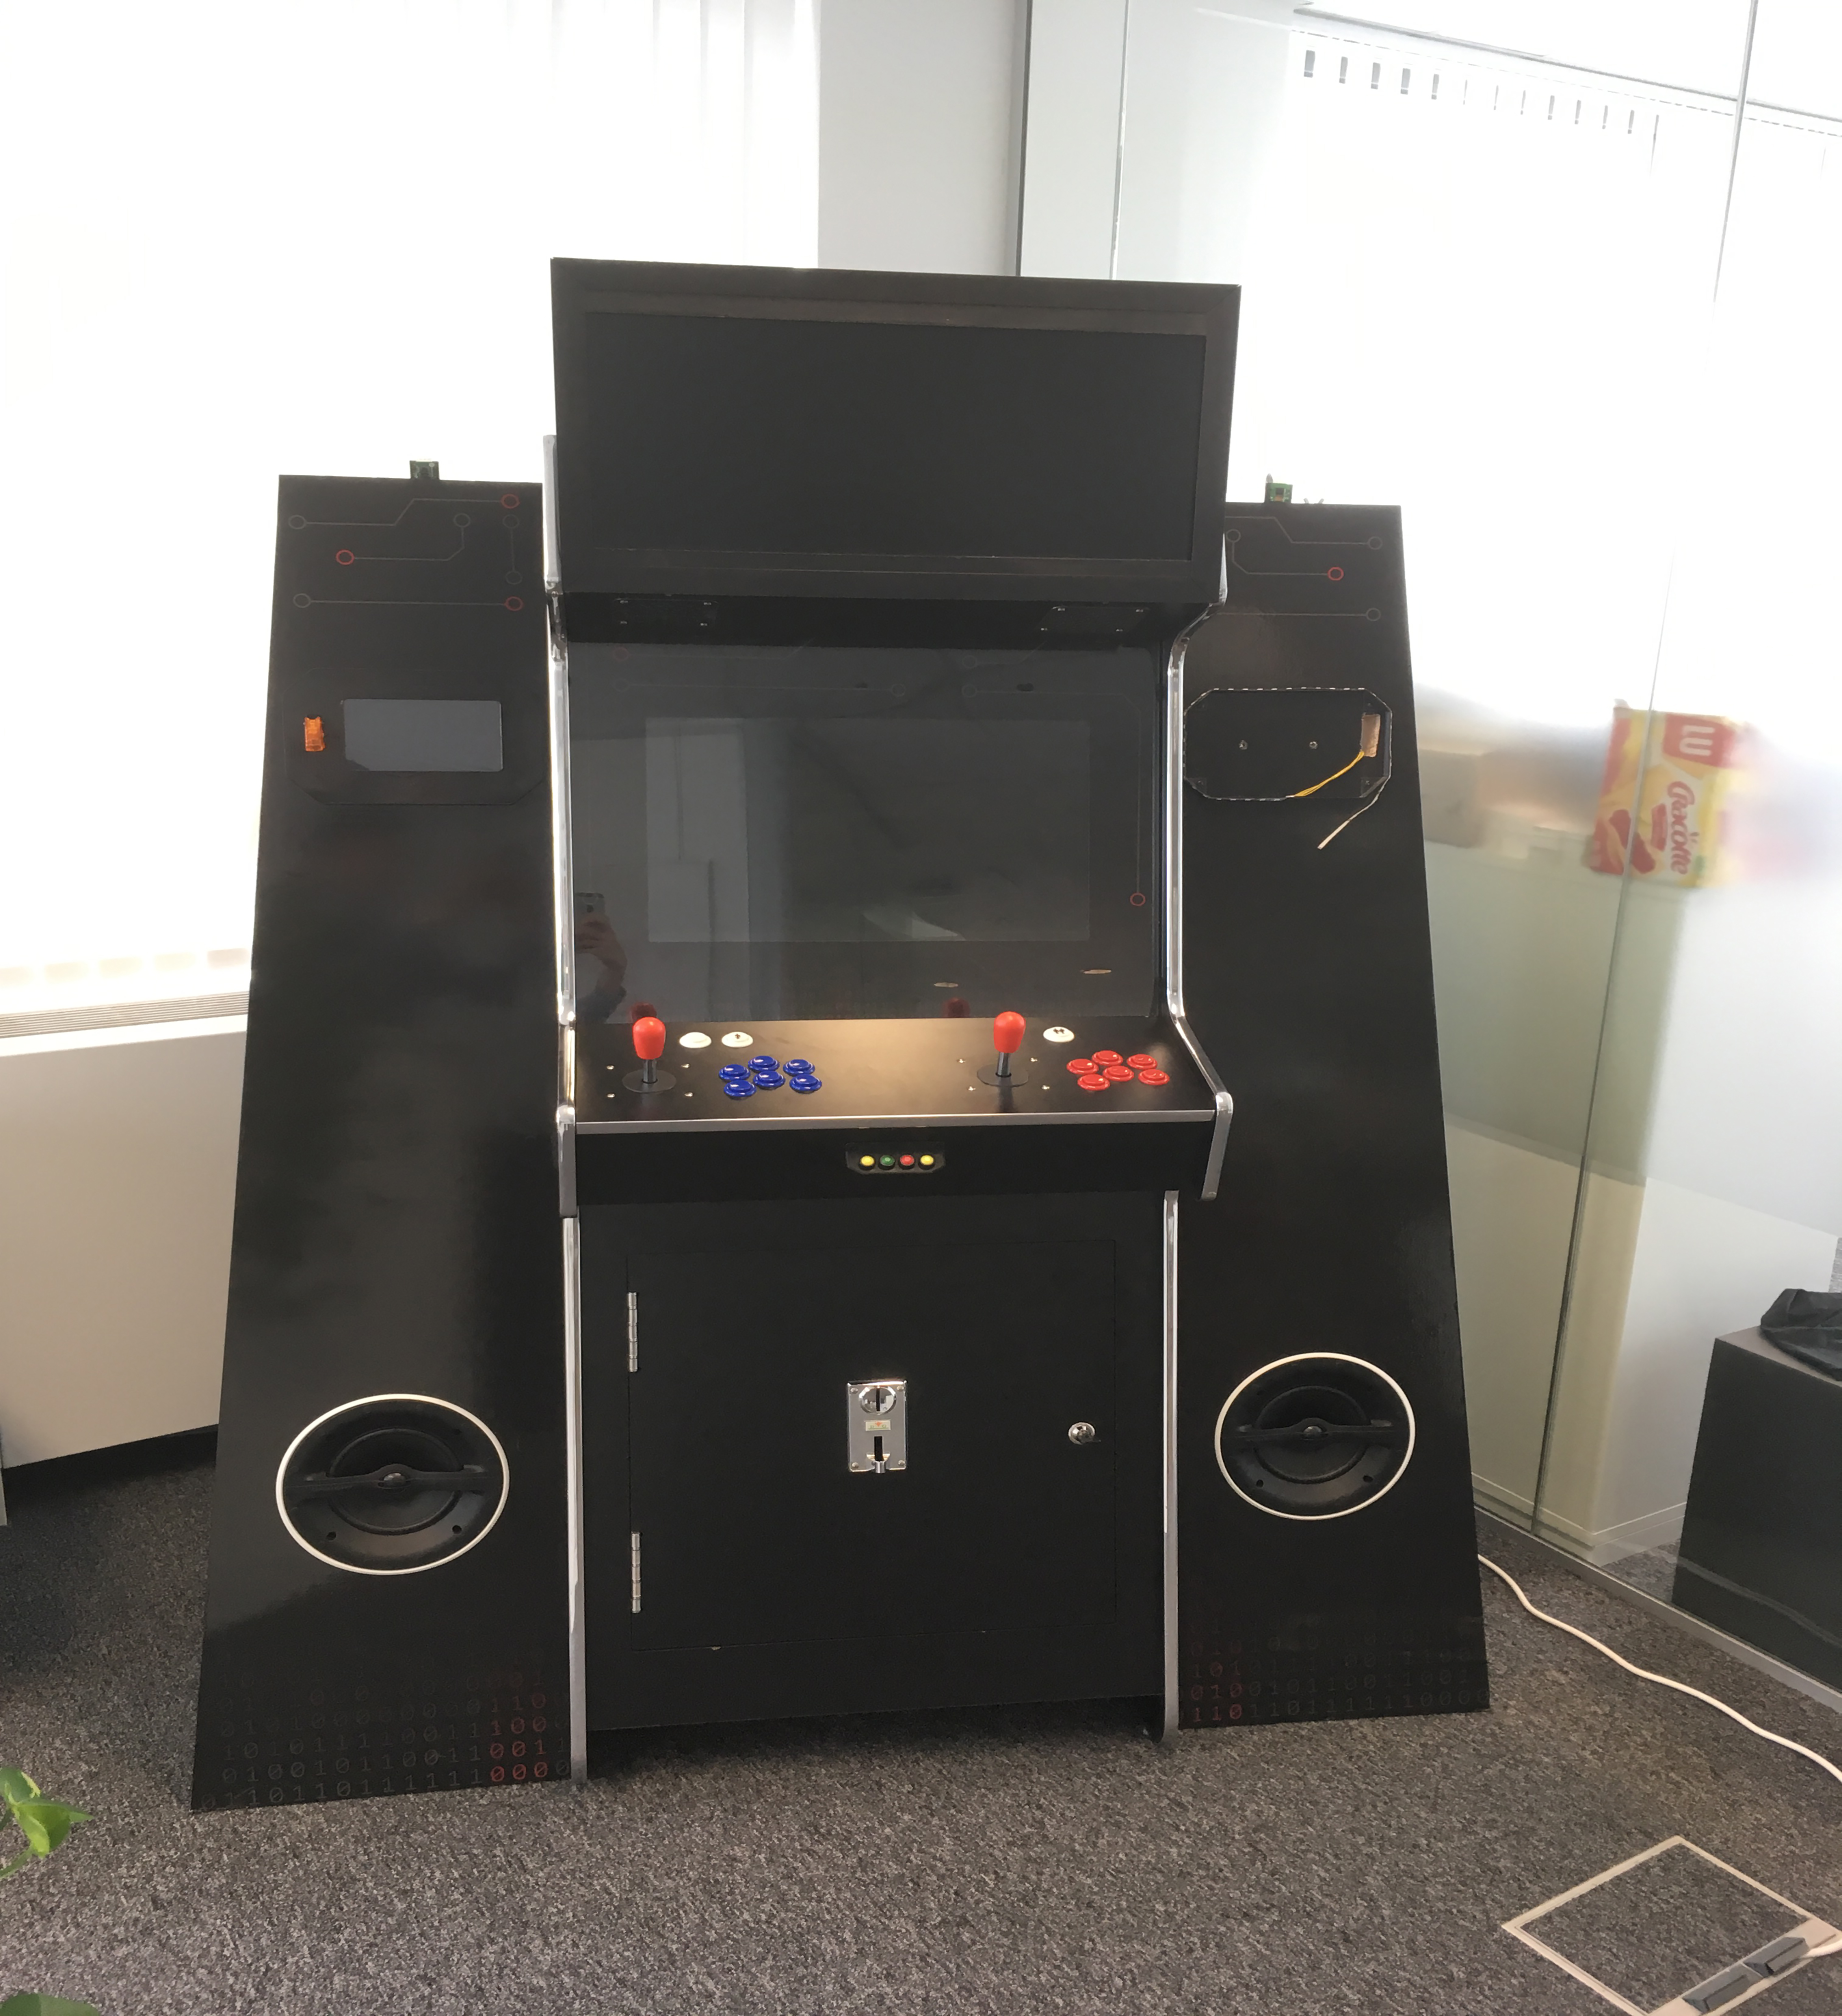
\includegraphics[width=0.6\textwidth]{img/machine}
	\caption{De arcade machine van ToThePoint}
	\label{fig:arcademachine}
\end{figure} ToThePoint zal het eerste bedrijf zijn die AI in een arcademachine zal verwerken. Aangezien er nog geen andere gelijkaardige voorbeelden te vinden zijn zal er van bij het begin onderzoek gedaan moeten worden. Hoe pakken we dit het best aan en verklaren waarom die aanpak de beste is. De spelletjes worden bestuurd door zes knoppen en een joystick. Aan de hand van de snelheid van een spel, het aantal keer een knop ingedrukt wordt of het aantal joystickbeweging. Aan de hand van deze inputparameters zullen we kunnen onderscheiden welk spel de gebruiker aan het spelen is. Er bestaan al veel verschillende soorten algoritmen maar deze zijn niet allemaal geschikt voor deze casus en daar zal dus aan gewerkt moeten worden. 

Artificiële intelligentie is hot en zo worden er allerlei beginnende frameworks ontwikkeld die reeds geïmplementeerde algoritmen bevatten of het eenvoudiger maken om ermee te starten. 
Tensorflow is een populair framework ontwikkeld door Google en gemaakt in Python. Dit wordt gebruikt in verschillende producten van Google zoals Google's stemherkenning, Google vertaler, het zoeken op afbeeldingen, etc.
TensorFlow maakt gebruik van deep learning-algortimen of neurale netwerken. De voorbeelden van Tensorflow gaan bijna uitsluitend over image recognition maar het is mogelijk om andere applicaties ermee te ontwikkelen. Dat is dan ook de reden dat Google dit framework open source heeft gemaakt zodat ze kunnen zien waar er nog verbeteringen aangebracht kunnen worden en wat er nog allemaal mogelijk is. \autocite{GooglesTensorflow}
Een ander interessant framework is het accord-framework \autocite{accord} die volledig ontwikkeld is in C\#. Hierin zitten veel geïmplementeerde algoritmen die dan kunnen gebruikt worden door derden om een eigen applicatie met artificiële intelligentie te ontwikkelen. 

Er zijn al enkele vergelijkingen over algoritmen geweest. Eén daarvan is een vergelijkende studie van verschillende gesuperviseerde algoritmen \autocite{vergelijkingSupervised}. Daarin was te vinden dat het support vector machine-algoritme tot de beste gesuperviseerde algoritmen behoort. Doorheen deze bachelorproef zullen we dit algoritme bespreken en vergelijken met logistische regressie. Er is wel vermeld dat de resultaten afhankelijk zijn van welke dataset gebruikt wordt. Misschien zal in deze casus logistische regressie de voorkeur krijgen.

\section{Probleemstelling en Onderzoeksvragen}
\label{sec:onderzoeksvragen}

%% TODO:
%% Uit je probleemstelling moet duidelijk zijn dat je onderzoek een meerwaarde
%% heeft voor een concrete doelgroep (bv. een bedrijf).
%%
%% Wees zo concreet mogelijk bij het formuleren van je
%% onderzoeksvra(a)g(en). Een onderzoeksvraag is trouwens iets waar nog
%% niemand op dit moment een antwoord heeft (voor zover je kan nagaan).

Machine learning is momenteel aan het boomen. Dit wordt nu zeer veel toegepast voor online advertising met Google en Facebook als de leiders. Maar ook meer en meer bedrijven beginnen zich te verdiepen in artificiële intelligentie. ToThePoint is zich hierop ook aan het voorbereiden. Door middel van een funproject willen ze zich zoveel als mogelijk verdiepen in allerlei gebieden binnen de informatica.

Men heeft een arcademachine gekocht die ze volledig gaan customizen met verschillende technologieën. Daar kunnen ze al hun kennis op loslaten. Inclusief de kennis die ze zullen opdoen via deze bachelorproef. Hierdoor zullen ze dus iets bijleren over artificiële intelligentie en dit dan ook kunnen toepassen. Verder zal de machine geplaatst worden op allerlei jobbeurzen om gegevens van studenten op te slaan bijvoorbeeld. Het nut dit funproject is niet alleen om bij te leren maar de machine zal ook dienen als referentie naar klanten toe. Zo kan ToThePoint aantonen tot wat ze instaat zijn. 

In deze bachelorproef wordt er een vergelijkende studie gemaakt tussen twee verschillende algoritmen. Het beste algoritme zal dan uiteindelijk geïmplementeerd worden in de arcade machine. Je kan hier heel ver in gaan. De voorspellingen kunnen bijvoorbeeld gemaakt worden door welke de meest gebruikte knop is of joystick beweging. Maar ook door de snelheid waarmee knoppen bediend worden en de frequentie van dezelfde knop, is het spel eerder een multiplayer spel of niet,...  Aan de hand van deze verschillende factoren is het mogelijk om voorspellingen te doen. Als het nog verder uitgewerkt wordt kan er naar toetsencombinaties gekeken worden maar dit is te verregaand voor deze bachelorproef. Er zal vooral gefocust worden op hoe een goed algoritme gekozen wordt. Het stappenplan dat uitgewerkt zal worden kan dan ook toegepast worden op toekomstige projecten. Uiteindelijk zullen we een antwoord hebben op de vraag welk algoritme het meest geschikt is om voorspellingen te doen op een arcademachine.



\section{Opzet van deze bachelorproef}
\label{sec:opzet-bachelorproef}

%% TODO: Het is gebruikelijk aan het einde van de inleiding een overzicht te
%% geven van de opbouw van de rest van de tekst. Deze sectie bevat al een aanzet
%% die je kan aanvullen/aanpassen in functie van je eigen tekst.

De rest van deze bachelorproef is als volgt opgebouwd:

In Hoofdstuk~\ref{ch:methodologie} wordt de methodologie toegelicht en worden de gebruikte onderzoekstechnieken besproken om een antwoord te kunnen formuleren op de onderzoeksvragen.

%% TODO: Vul hier aan voor je eigen hoofstukken, één of twee zinnen per hoofdstuk

In Hoofdstuk~\ref{ch:conclusie}, tenslotte, wordt de conclusie gegeven en een antwoord geformuleerd op de onderzoeksvragen. Daarbij wordt ook een aanzet gegeven voor toekomstig onderzoek binnen dit domein.

